\documentclass[a4paper, 11pt]{article}
\topmargin=-0.45in
\evensidemargin=0in
\oddsidemargin=0in
\textwidth=6.5in
\textheight=9.0in
\headsep=0.25in 


% Margins
\topmargin=-0.45in
\evensidemargin=0in
\oddsidemargin=0in
\textwidth=6.5in
\textheight=9.0in
\headsep=0.25in 

%package usage
\usepackage[table,xcdraw,usenames,dvipsnames]{xcolor}
\usepackage[colorlinks=true, citecolor=blue, linkcolor=MidnightBlue,urlcolor=MidnightBlue]{hyperref}
\usepackage[english]{babel}
\usepackage[latin1]{inputenc}
\usepackage{indentfirst}
\usepackage{enumitem}
\usepackage{colortbl}
\usepackage{longtable}
\usepackage{threeparttablex}
\usepackage{etoolbox}
\usepackage{rotating}
\usepackage{array}
\usepackage{multirow}
\usepackage{pdflscape}
\usepackage{makecell}
\usepackage{tablefootnote}
\usepackage{makecell}
\usepackage{tabularx}
\usepackage{csquotes}
\usepackage{amssymb}
\usepackage{pifont}
\usepackage{amsmath}
\usepackage{comment}
\usepackage{flafter} 
\usepackage{dcolumn} 
\usepackage{natbib}
\usepackage{rotating}	
\usepackage{amsthm}
\usepackage{graphicx}
\usepackage{amssymb}
\usepackage{adjustbox}
\usepackage{tcolorbox}
\usepackage{lipsum}
\usepackage{tikz}
\usepackage{tabularx}
\tcbuselibrary{skins,breakable}
\usetikzlibrary{shadings,shadows}
\usepackage{threeparttable}
\usepackage{subfig}
\usepackage{setspace}
\usepackage{booktabs}
\usepackage{placeins}
\usepackage{enumitem}
\usepackage[encoding,filenameencoding=utf8,extendedchars,space]{grffile}
\newcommand{\addfig}[2]{\begin{center}
			\includegraphics[width=#1\textwidth]{#2}
	\end{center}
}

%\usepackage[capposition=top]{floatrow}
%\usepackage[colorinlistoftodos]{todonotes}
\newcommand{\expect}[2]{\mathbb{E}_{#2}\left(#1\right)}
\newcommand{\explaino}[2]{\overbrace{#1}^{\text{\textbf{#2}}}}

\newtheorem{theorem}{Theorem}[section]
\newtheorem{corollary}{Corollary}[theorem]
\newtheorem{proposition}[theorem]{Proposition}

\newcommand{\alert}[1]{{\textbf{\color{red}#1}}}
%general commands
\newcommand{\beqns}{\begin{eqnarray*}}
\newcommand{\eeqns}{\end{eqnarray*}}
\newcommand{\beqn}{\begin{eqnarray}}
\newcommand{\eeqn}{\end{eqnarray}}
\newcommand{\benu}{\begin{enumerate}}
\newcommand{\eenu}{\end{enumerate}}
\newcommand{\bitem}{\begin{itemize}}
\newcommand{\eitem}{\end{itemize}}
\newcommand{\smallGap}{\vspace{.25cm}}
\newcommand{\oemph}[1]{\textbf{\orange{#1}}}

\newenvironment{block}[1]{%
	\tcolorbox[beamer,%
	noparskip,breakable,
	colback=LightGreen,colframe=DarkGreen,%
	colbacklower=LimeGreen!75!LightGreen,%
	title=#1]}%
{\endtcolorbox}


\newcommand{\sym}[1]{\rlap{#1}}% Thanks David Carlisle

\usepackage{siunitx}
\sisetup{
	detect-mode,
	group-digits		= false,
	input-symbols		= ( ) [ ] - +,
	table-align-text-post	= false,
	input-signs             = ,
}

%mathematical commands

\newcommand{\cov}{\text{cov}}
\newcommand{\var}[1]{\text{var}\left(#1\right)}
\newcommand{\red}[1]{{\color{red}#1}}
\newcommand{\blue}[1]{\color{blue}{#1}}
\newcommand{\green}[1]{{\color{Green}#1}}

\newcommand{\vs}{\vspace{1mm}}
\usepackage{framed}
\definecolor{shadecolor}{gray}{0.875}
\specialcomment{answer}{\begin{shaded}}{\end{shaded}}
\newcommand{\PreserveBackslash}[1]{\let\temp=\\#1\let\\=\temp}
\newcolumntype{C}[1]{>{\PreserveBackslash\centering}p{#1}}
\newcolumntype{R}[1]{>{\PreserveBackslash\raggedleft}p{#1}}
\newcolumntype{L}[1]{>{\PreserveBackslash\raggedright}p{#1}}
\newcommand{\thesispath}{..}
\usepackage{titlesec}
\usepackage{breakurl}
\urlstyle{same}
\usepackage{float}
\usepackage{natbib}

\usepackage{listings}
\usepackage{color}
\usepackage{upquote}

\definecolor{dkgreen}{rgb}{0,0.6,0}
\definecolor{gray}{rgb}{0.5,0.5,0.5}
\definecolor{mauve}{rgb}{0.58,0,0.82}



\onehalfspacing

%
%\newif\ifoptionSolution
%
%
%\optionSolutiontrue
%
%\ifoptionSolution
%\newcommand{\solution}[1]{{\textbf{\red{Solution:}} #1}}
%\else
%\newcommand{\solution}[1]{{#1}}
%\fi


\newcommand{\questionpoints}[1]{
	\par\noindent\textbf{[#1 mark(s)]}
}

\title{\large{\textbf{ECNM10112: Applied Labour Economics}}}
\author{\textbf{Regression Discontinuity Design (RDD) notes}}
\date{}
\begin{document}
	\maketitle
	
	As the name suggests, Regression Discontinuity Design is an empirical strategy that exploits discontinuities in the data to credibly establish causality and estimate treatment effects.
	
	
	Rules, policies, or traditions often introduce arbitrary cutoffs that affect the probability of receiving some treatment of interest. For example:
	\bitem 
		\item In many countries, you can start receiving your pension only after you turn 65 years old.
		\item Tax systems often have cutoffs that introduce discontinuities on your tax rate. For example, currently  in the UK you pay 0\% over all income below \textsterling12,750 but you pay 20\% over income between \textsterling12,571 and \textsterling50,270.
		\item Income thresholds often determine your ability to access government aid. For example, suppose only students whose parents make \textsterling 15,000 or less can get access to free school meals.
		\item Schools in Israel often split classes with more than 40 students \citep{Angrist1999a}. That is, if there are 40 students in fourth grade they stay as a single class. However, if a new student arrives then the school splits fourth grade into two classes.
	\eitem  
	
	RDD exploits the arbitrariness of these cutoffs to estimate treatment effects. 
	
	\section{A simple example}
	
	To fix ideas, suppose that you are interested in determining the effect of free school meals on student achievement. Your first idea is to run the following regression:
	\beqn
		\label{reg:school}
		score_i=\alpha + \tau school\_meal_i+u_i
	\eeqn
	where $score_i$ is some measure of student achievement and $school\_meal_i$ is a dummy equal to one if the student receives free school meals. Here, you are interested in estimating $\tau$, the free-meal treatment effect.
	
	Regression \eqref{reg:school} is unlikely to give us an unbiased treatment effect estimate because chances are that eligibility for school meals is correlated with a host of unobserved factors that also determine student achievement, that is $E( school\_meal\_i,u_i)\neq 0$. For example, kids receiving subsidised school meals might be attending worse schools, live in worse neighbourhoods, etc.
	
	However, suppose that after extensive research of the government rules, you discover the following:\footnote{The eligibility rule in this example is very extreme. In practice, rules are often less stringent. For example, rather than going from 100\% subsidy to zero, there can be more bands of income and subsidy that generate a more gradual decline in the levels of subsidy.}
	\bitem
		\item All students whose household income is \textsterling12,000 or less get free school meals.
		\item All students whose  household income is greater than \textsterling12,000 must pay meals in full.
	\eitem 
	The basic intuition of RDD is that this rule introduces differences in treatment for people that are similar in all other respects. We often worry that a simple comparison of outcomes between treated and control students will generate biased estimates. Students paying meals in full are richer and probably have access to better resources which would bias us against finding an effect even if there is one. 
	
	 However, what if we compare the outcomes of students with incomes just below and just above the 12,000 cutoff? Chances are that students whose parental income is \textsterling12,000 are very similar to those whose parental income is \textsterling12,001. An additional pound of income is certainly unlikely to give students access to better resources. But students just below 12,000 get free meals, while those just above do not. Therefore, if the \textsterling12,000 students have higher scores than the  \textsterling12,001 students, we can credibly argue that these differences are caused by the free school meals.
	
	\begin{figure}[!h]
\centering
\caption{RDD in a graph}
\label{fig:figure_1}
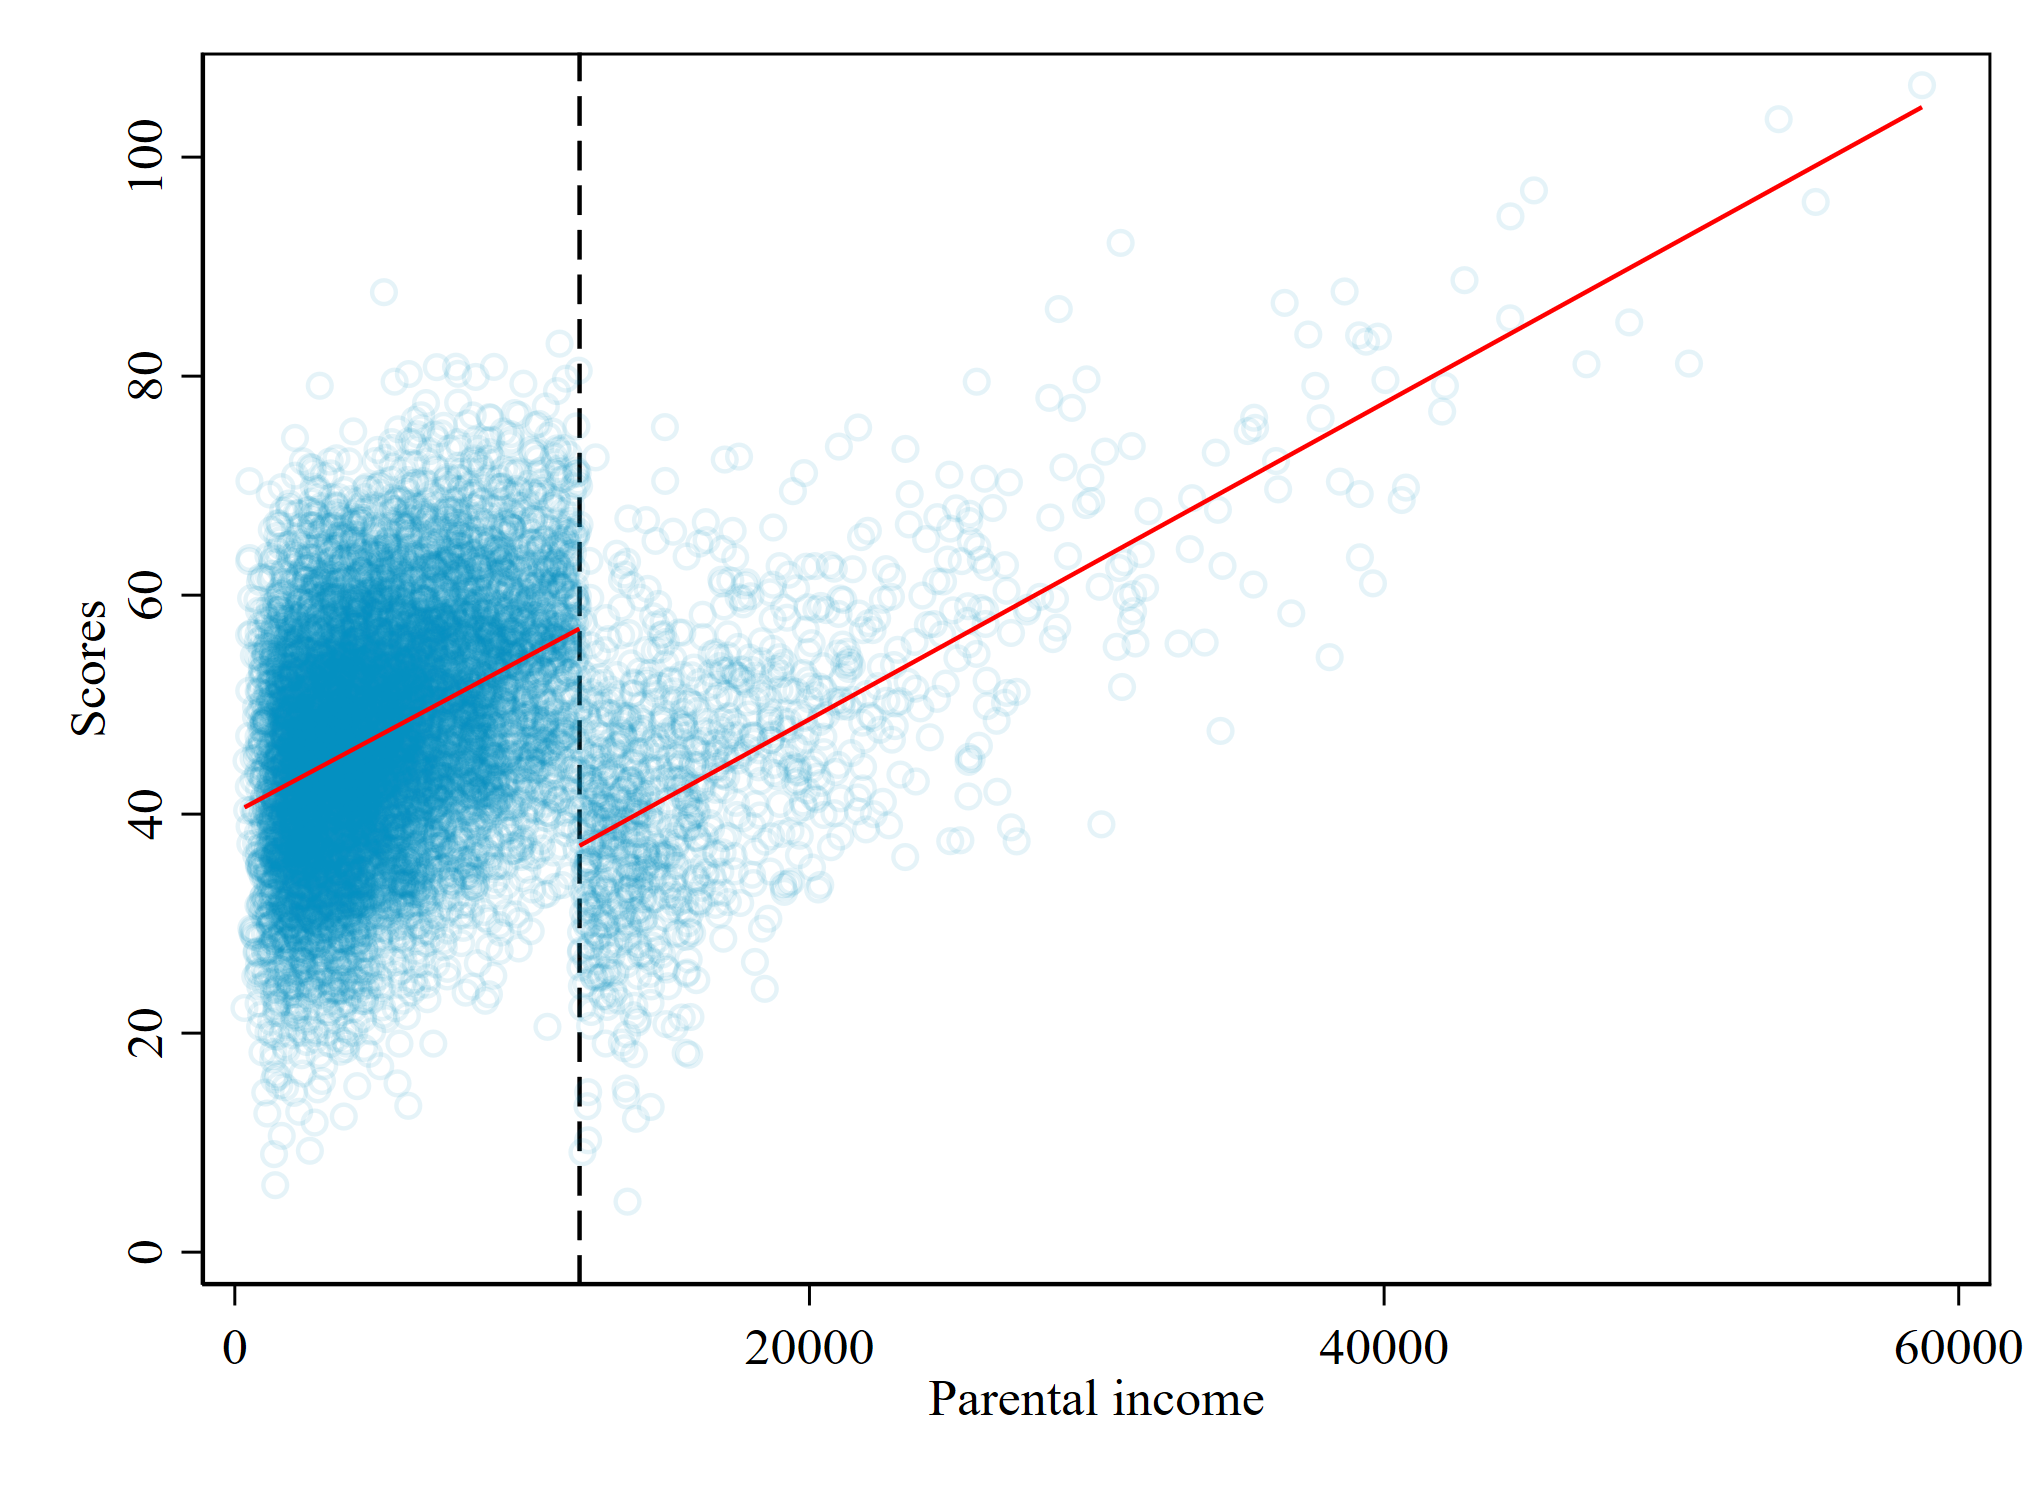
\includegraphics[width=.5\textwidth]{./figure_1}
\par \begin{minipage}[h]{\textwidth}{\scriptsize\textit{Notes:} Vertical line denotes \textsterling 12,000. Figure generated on 23 Sep 2024 at 18:26:33.}\end{minipage}
\end{figure}

	
	Figure \ref{fig:figure_1} illustrates this argument graphically. The figure plot the relationship between students' scores and parental income for some fictional data. Unsurprisingly, there is a positive relationship between parental income and student achievement. However, note that there is a discontinuity at \textsterling 12,000. Students with incomes just below \textsterling12,000 have higher scores than those with income just above \textsterling12,000. Because, all students to the left of this point get a free meal, while those to the right don't, the discontinuity in achievement is --presumably-- caused by the free meal. 
	
	\section{Estimating treatment effects using RDD}
	We can use regressions to estimate the treatment effect illustrated in Figure \ref{fig:figure_1}. To do so, define the free-meal eligibility rule dummy:
	\beqns
		D_i&=&\left\{\begin{array}{cc}
			1, &parental\_income_i\leq12,000\\
			0, &parental\_income_i>12,000
		\end{array}\right.
	\eeqns
	
	In RDD parlance parental income is called the \emph{the running variable}, i.e. the variable that generates the discontinuity in treatment status. We can estimate the treatment effect of the free meal with the regression:
	\beqn
		\label{rdd_linear}
		y_i&=&\alpha_0+\tau D_i +\beta_1 parental\_income_i+u_i
	\eeqn
	here $\tau$ provides an estimate of the size of the discontinuity at \textsterling 12,000 in Figure \ref{fig:figure_1}. Intuitively, $\tau$ is estimated by comparing the scores of students just below and just above the 12,000 cutoff. Therefore, $\tau$ will be an unbiased estimate of the (local) treatment effect whenever students that are just below and just above the cutoff are similar in all other respects. \textbf{This is the key identifying assumption in RDD: outcomes for students on each side of the cutoff would have been the same in the absence of the free meal.}
	\subsection{Allowing for more flexibility between the dependent and the running variables}
	Regression \eqref{rdd_linear} is very simple, but it imposes a lot of restrictions on the relationship between scores are parental income: it must be linear and it must be the same on both sides of the discontinuity. However, the relationship between these variables could be non-linear or change at the discontinuity. Figure \ref{fig:figure_2} Panel (a) gives an example where there is a non-linear relationship between the variables. Panel (b) gives an example of a linear relationship but with different slopes (different functional form) on each side of the discontinuity.
	
	\begin{figure}[!h]
\centering
\caption{RDD and functional form}
\label{fig:figure_2}
\subfloat[Non-linear relationship with the running variable]{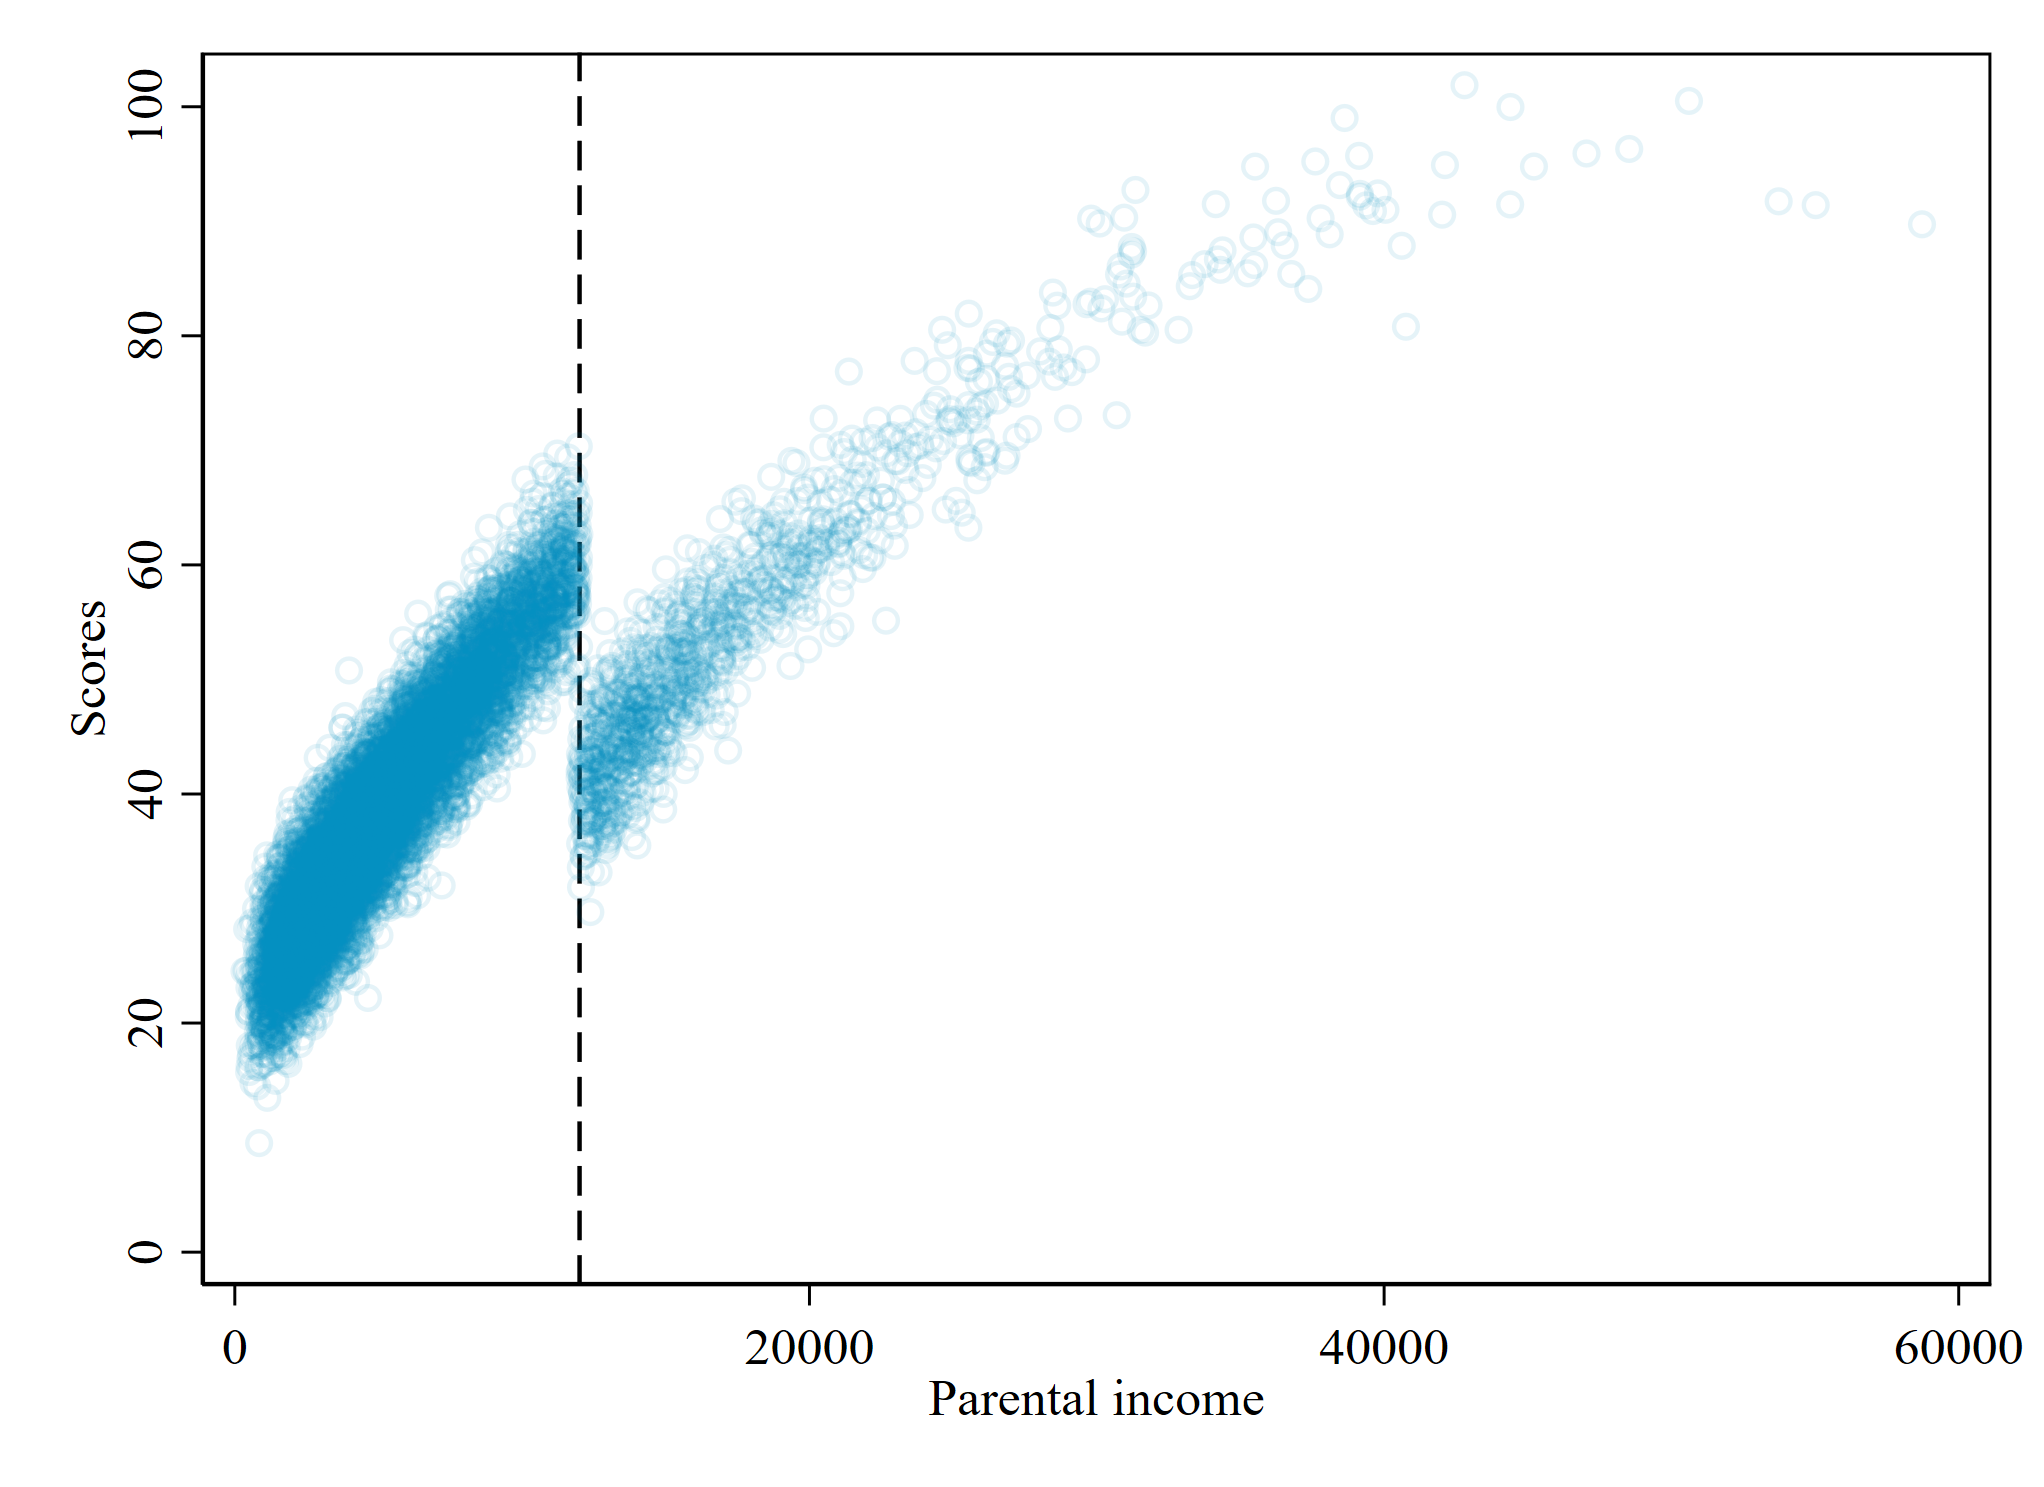
\includegraphics[width=.5\textwidth]{./figure_2_a}} \subfloat[Different function on each side of the discontinuity]{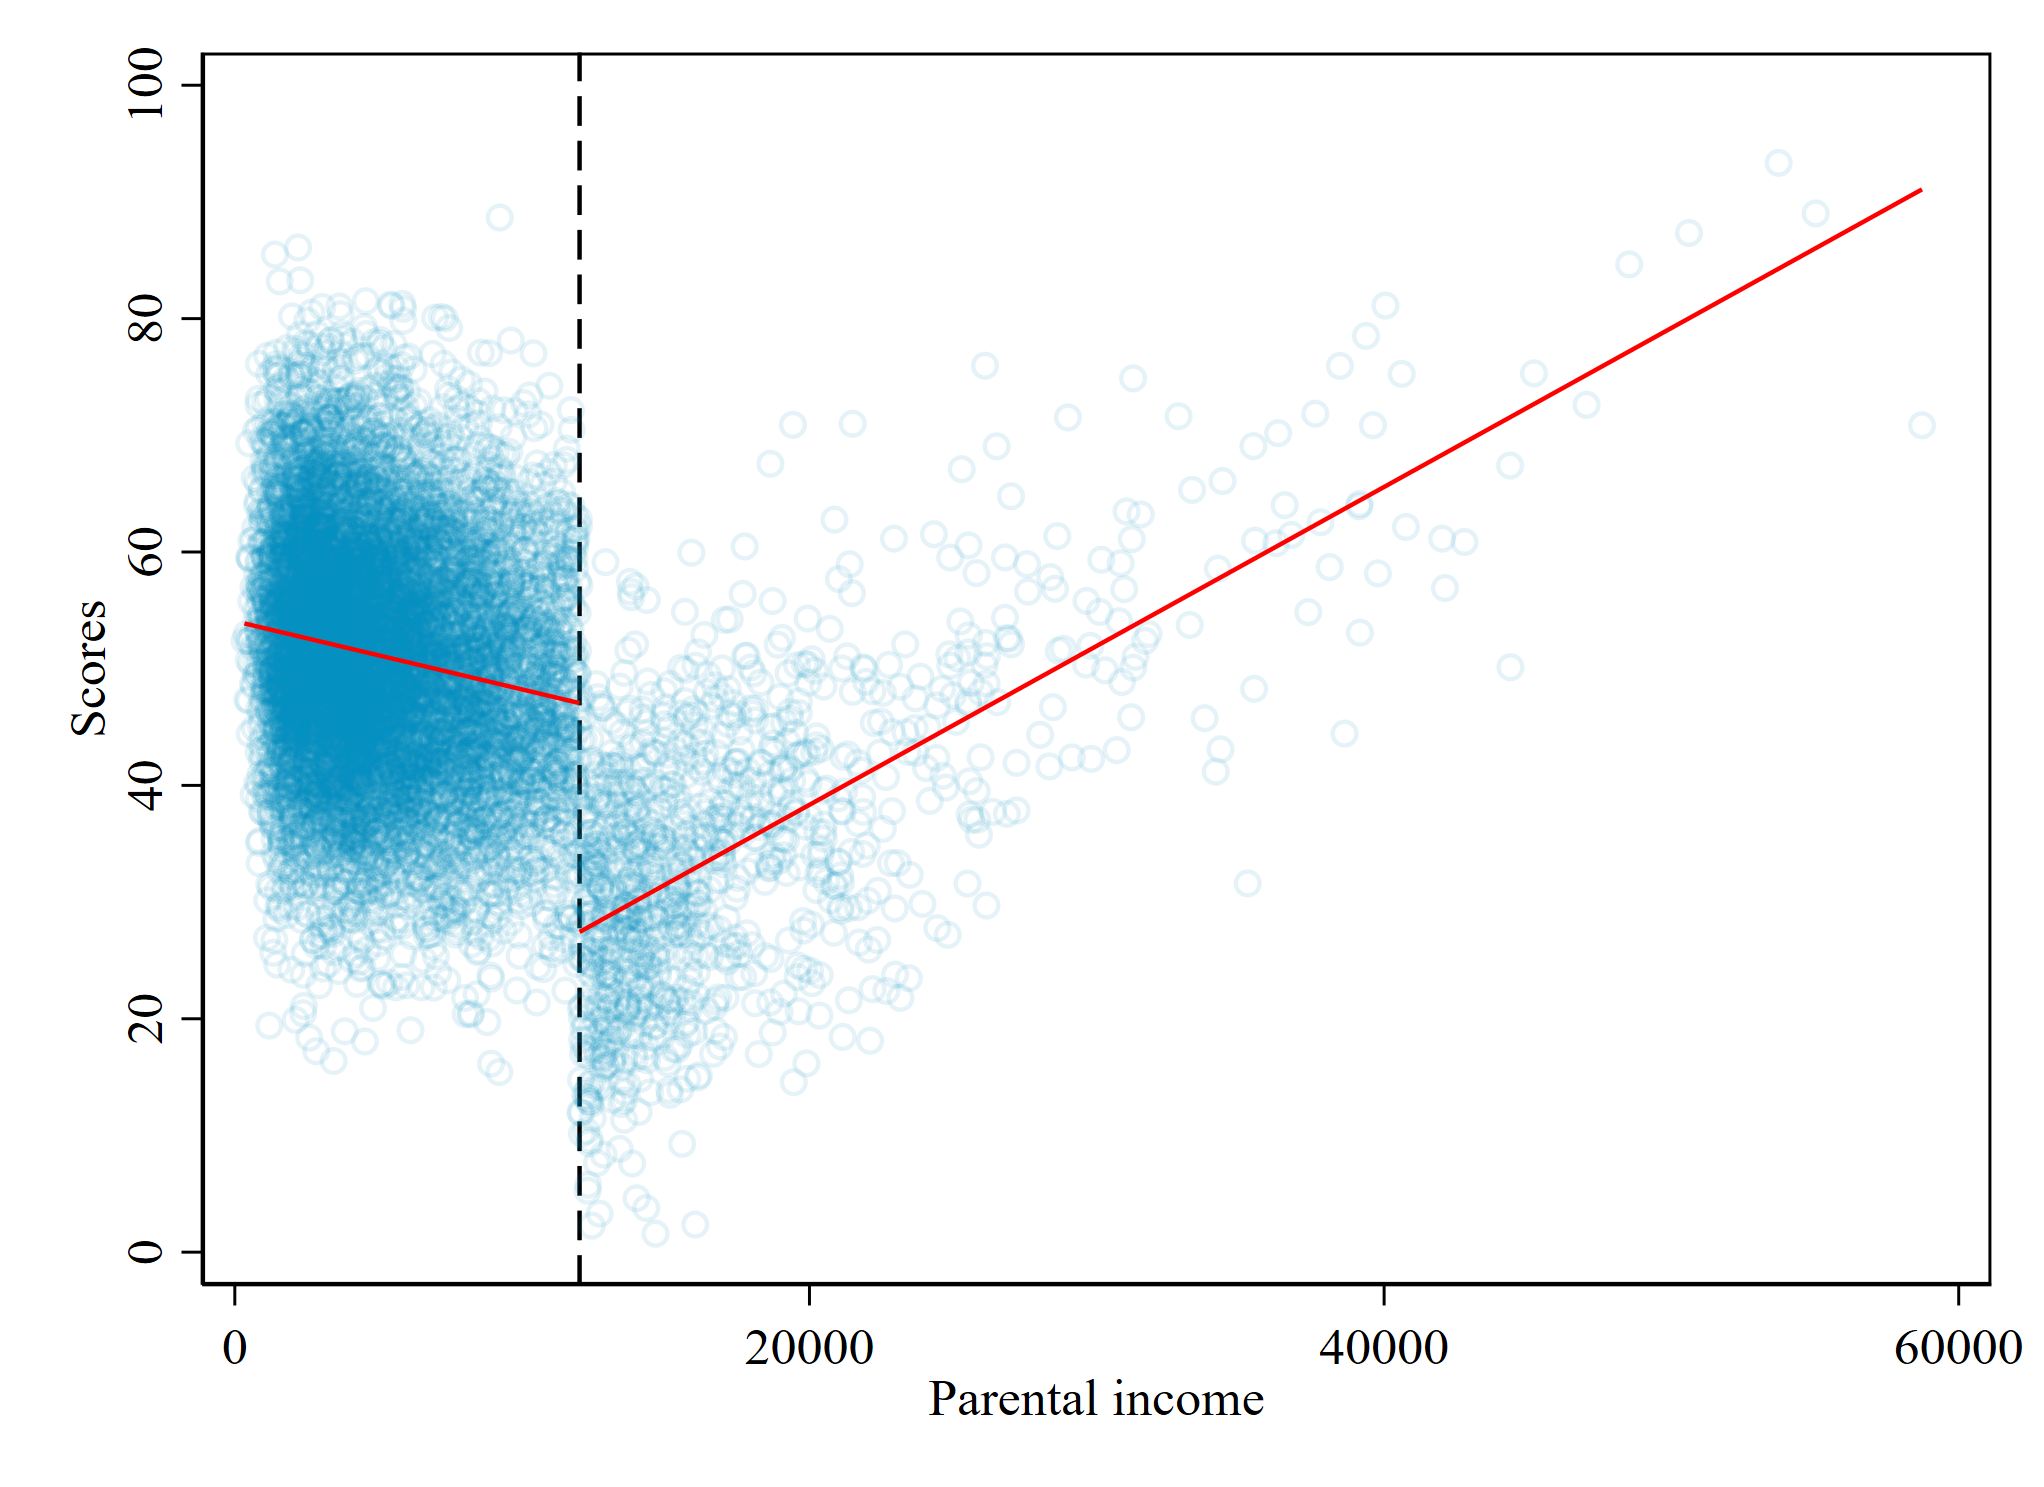
\includegraphics[width=.5\textwidth]{./figure_2_b}} \\ 
\par \begin{minipage}[h]{\textwidth}{\scriptsize\textit{Notes:} Vertical line denotes \textsterling 12,000.}\end{minipage}
\end{figure}


	These situations are very easy to accommodate. Flexible functional forms can be easily incorporated by using polynomials of the running variable. For instance, below is a RDD specification using a quadratic polynomial:
	\beqn
	\label{rdd_quad}
	y_i&=&\alpha_0+\tau D_i +\beta_1 parental\_income\_i+\beta_2 parental\_income_i^2+u_i
	\eeqn
	here, $\tau$ gives us the treatment effect estimate. 
	
	The specification above imposes the same functional form on each side of the discontinuity. A simple modification relaxes this restriction:
	\beqn
	\label{rdd_diff}
	y_i&=&\alpha_0+\tau D_i +\beta_1 parental\_income\_i+\beta_2 parental\_income_i^2+\notag\\
		&&\beta_3 D_i\times (parental\_income\_i-12,000)+\beta_4D_i\times (parental\_income\_i-12,000)^2+u_i
	\eeqn
	the two additional terms allow the relationship between scores and income to switch at 12,000. Again, the estimate for $\tau$ will be treatment effect estimate.
	\bibliographystyle{apalike}
	\bibliography{../../../../../../0_central_library/Papers/library}{}
\end{document}
